\chapter{Methodology}

\section{Research Methodologies}
In the early stages of the project, qualitative research was carried out by gathering data from the client about the requirements for the project and the procedures the company uses explaining why it was needed.This was vital in order to gain an in-depth understanding of the problem at hand. Contact was quite frequent with the client until all sides were understanding of the problem domain. Areas such as the technologies to be used, workload to be undertaken and methodologies used in the project were all decided in this phase. When the list of requirements were gathered these were again reviewed by the client in a meeting to ensure that all aspects required for the project were covered in these requirements.\par
As the project progressed the focus on research shifted from qualitative to quantitative research. The client would be sent video updates or physical prototypes to be tested by themselves and associated parties by which feedback was received. This feedback was then used to make desired adjustments to the application. It also helped create an understanding of users' perspectives of the application.
\newpage

\section{Software Development Methodologies}
The software testing strategy used throughout the project life cycle was Extreme Programming. Extreme Programming is a form of agile development that is carried out in sprint cycles. Agile development allows for changing requirements in a project due to its incremental nature. Due to consistent contact with the client, changes were taken into account quite frequently. The agile development style allowed for these changes to have minimal impact on the project.\par
Usage of an agile methodology was evident before development commenced. Extreme Programming was chosen due to its short sprint cycles, allowance of test driven development and emphasis on continuous integration. It also accounts for priority development and allows these priorities to be changed. Extreme programming is very adaptable which is suited to an integration heavy project such as this.

\begin{figure}[h!]
 	\caption{Extreme Programming lifecycle}
	\label{image:xp}
 	\centering
 	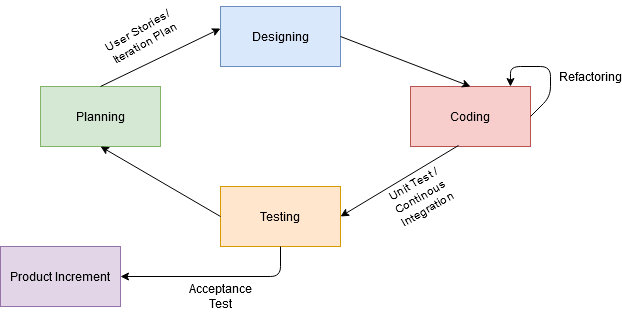
\includegraphics[width=0.9\textwidth]{Images/XP Cycle.png}
\end{figure}	
\newpage
\section{Testing Methodologies}
Testing was carried out at the end of every integration and sprint within the project. This allowed for continuous testing throughout the development lifecycle. This type of frequent testing was necessary in a project which is very integration driven. This allowed for early bug prevention and as well as ensuring all new integrations worked in collaboration with previous integrations. \par
Testing tools were also looked at as part of the testing methodology. These were vital in order to carry out testing to a high standard. Testing tools such as Postman for testing the API and PyTest for unit testing on the server side were both documented for use from the beginning of the project. Selenium was documented to test components when they were in a state where they were able to carry out the required functionality, which could then be used to conduct integration testing later in the project.